\chapter{Planificaci\'on del Proyecto de Software}
En el presente cap\'itulo se brinda al cliente un modelado inicial del software con todos los requerimientos anteriormente descritos, puliendo de esa manera los criterios mediante los cuales se trabaja, el tiempo estimado del desarrollo del proyecto y los costos preliminares.

\section{Alcances Proyecto de Software}
\begin{itemize}
	\item Obtener un software dotado de 4 diferentes componentes que permitan el correcto manejo de la necesidad de gesti\'on de inventario del cliente; estos componentes ser\'an: \textit{Informaci\'on del Medicamento, Cantidades de medicamentos, Informaci\'on de Proveedores, Notificaciones por vencimiento.}
	\item Garantizar al cliente la reducci\'on del tiempo en la busqueda de medicamentos para las respectivas ventas de los mismos y as\'i hacer m\'as eficiente el proceso de gesti\'on de inventario de la droguer\'ia.
\end{itemize}
\newpage
\section{Objetivos Proyecto de Software}
\begin{itemize}
	\item Implementar un m\'odulo de gesti\'on de inventario amigable y entendible para el cliente.
	\item Incorporar el producto final al hardware usado por el cliente de tal manera que este sea compatible por dicho hardware para un acorde manejo, garantizando que el cliente no necesite invertir tiempo en aprender m\'as de lo necesario para su uso.
	\item Proveer al usuario la facilidad del control y manejo de sus medicamentos durante su jornada laboral.
\end{itemize}
\section{Metodolog\'ia Proyecto de Software}
La metodolog\'ia que se utilizar\'a para este proyecto ser\'a la metodolog\'ia SCRUM, la cual se entiende como un marco de trabajo, en el que se aplican de manera regular un conjunto de buenas pr\'acticas para el trabajo de desarrollo y mantenimiento de manera colaborativa, en equipo de todo el software a trabajar para obtener el mejor resultado posible del proyecto.\\

Para el desarrollo se realiza de forma iterativa e incremental. Cada iteraci\'on, denominada Sprint, tiene una duraci\'on preestablecida de entre 2 y 4 semanas, obteniendo como resultado una versi\'on del software con nuevas prestaciones listas para ser usadas. En cada nuevo Sprint, se va ajustando la funcionalidad ya construida y se añaden nuevas prestaciones prioriz\'andose siempre aquellas que aporten mayor valor de negocio.\\

El sistema debe ser construido sobre la base de un desarrollo evolutivo e incremental, de manera tal que nuevas funcionalidades y requerimientos relacionados puedan ser incorporados afectando el c\'odigo existente de la menor manera posible; para ello deben incorporarse aspectos de reutilizac\'on de componentes.

\begin{center}
\begin{figure}[htb]
\centering
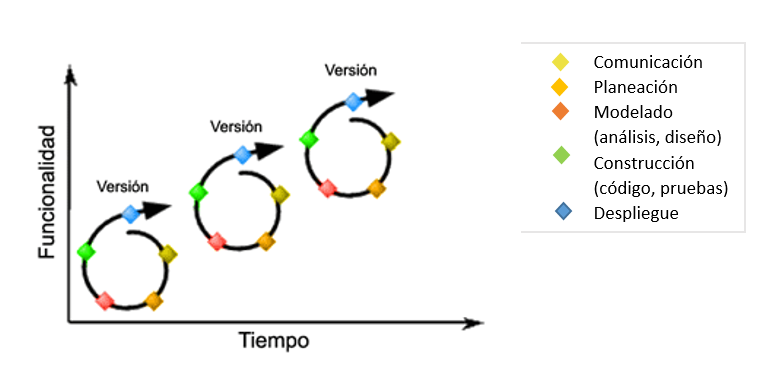
\includegraphics[width = 0.8\textwidth]{./capitulo4/img/modIncremental.png}
\caption{Modelo Evolutivo Incremental}
\end{figure}
\end{center}
\newpage

\section{Determinaci\'on de Recursos del Proyecto de Software}
\subsection{Recursos Humanos}
\begin{table}[h!]
	\begin{center}
		\begin{tabular}{|p{5cm} |p{5cm}|p{4cm}|} 
			\hline \textbf{Nombre} & \textbf{Perfil} & \textbf{Rol} \\
			\hline Edwin Garcia & Ingeniero de Sistemas & Desarrollador \\ 
			\hline Brian Rodr\'iguez & Ingeniero de Sistemas & Desarrollador \\
			\hline
		\end{tabular}
		\caption{Equipo de Desarrollo}
		\label{teamDevelop}
	\end{center}
\end{table}
%(Equipo de trabajo, perfiles y roles)
\subsection{Recursos Tecnologicos}
\subsubsection*{Hardware}
Se usaran dos computadores para el desarrollo del aplicativo.
\begin{table}[h!]
	\begin{center}
		\begin{tabular}{|p{7cm} |p{7cm}|} 
			\hline \textbf{Marca} &  HP 14\\
			\hline \textbf{Procesador} &  Intel Core i5\\
			\hline \textbf{RAM} &  8 Gb\\
			\hline \textbf{Disco Duro} &  700 Gb\\
			\hline \textbf{Sistema Operativo} &  GNU/Linux (Linux Mint)\\
			\hline
		\end{tabular}
		\caption{Referencias del Primer Computador}
		\label{equipoU}
	\end{center}
\end{table}
\newpage

\begin{table}[h!]
	\begin{center}
		\begin{tabular}{|p{7cm} |p{7cm}|} 
			\hline \textbf{Marca} &  HP ENVY 15 \\
			\hline \textbf{Procesador} &  Intel Core I7\\
			\hline \textbf{RAM} &  8 Gb\\
			\hline \textbf{Disco Duro} &  1 Tb\\
			\hline \textbf{Sistema Operativo} &  Windows 8.1\\
			\hline
		\end{tabular}
		\caption{Referencias del Segundo Computador}
		\label{equipoD}
	\end{center}
\end{table}
\subsubsection*{Software}
Se usar\'a el IDLE de Eclipse para el desarrollo del aplicativo (Mediante el lenguaje JAVA), de igual forma se usará Enterprise Architect 11 para la realizaci\'on del modelamiento en software del aplicativo.
\subsubsection*{Base de Datos}
Se usar\'a como motor de persistencia PgAdmin III, y a su vez el lenguaje mediante el cual se representar\'a la base de datos ser\'a PostgreSQL, haciendo conexi\'on con Eclipse.
\subsubsection*{Comunicaciones}

\subsubsection*{Ingenier\'ia Web}

%Hardware, Software, Aplicaciones y BD, Comunicaciones, Ingeniería Web

\subsection{Recursos Financieros} 
\textbf{PROBE}
\newline
Este método est\'a descrito en el libro PSP A Self-Improvement Process for Software Engineers, aunque es un poco complicado de seguir, por eso que mejor hacer un trabajo m\'as pr\'actico para tratar de enfocar el aprendizaje haciendo m\'as que diciendo.\\

Un proxy es una unidad de software que se puede identificar en un proyecto. Ejemplos de ello son las pantallas (User Interfaces), archivos, objetos, entidades l\'ogicas, funciones (Stores Procedures) y puntos de funci\'on. La representaci\'on se puede visualizar f\'acilmente a partir de las especificaciones del proyecto tales como documentos de requisitos. A continuaci\'on, se pueden traducir en l\'ineas de c\'odigo en funci\'on de los tamaños de los proxies hist\'oricos similares en proyectos de desarrollo anteriores. La l\'ineas de c\'odigo junto con cifras de productividad se pueden utilizar para predecir los recursos necesarios para un proyecto.\\

A continuaci\'on se muestra una tabla realizada mediante el m\'etodo PROBE (Proxy Based Estimation) el cual se utiliz\'o para elaborar la estimaci\'on en d\'ias trabajados por hombre para una cantidad requerida de proxys solicitados dentro del proyecto a realizar.

\begin{figure}[h!]
	\centering
	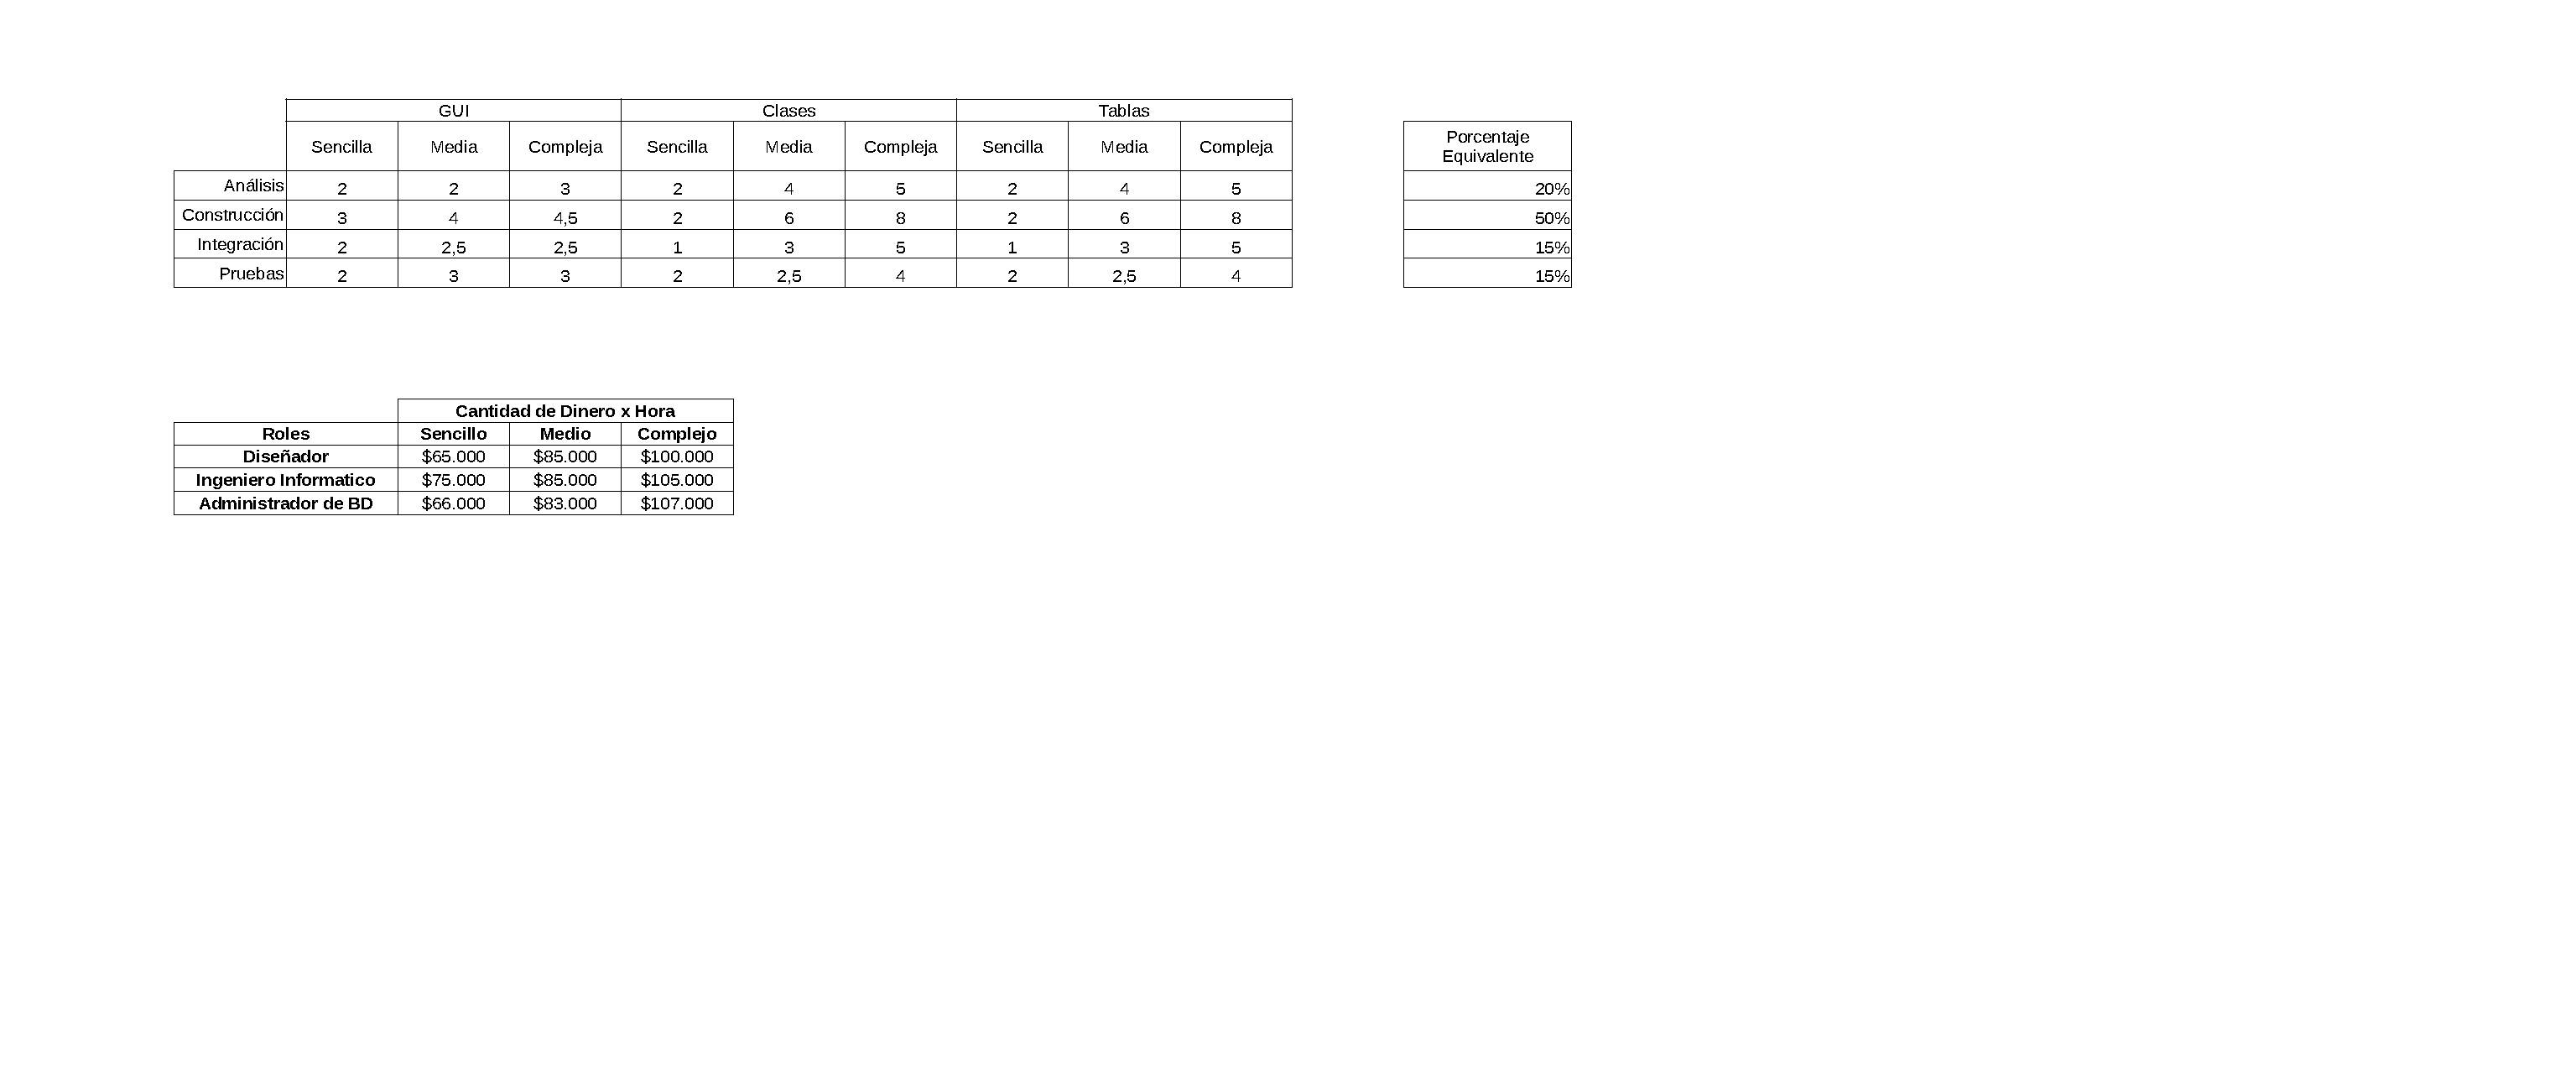
\includegraphics[width=1.2\linewidth]{libro/capitulo4/img/PROBE.pdf}
	\caption{Parametros para realizar la estimaci\'on}
\end{figure}
\newpage
\textbf{Estimaci\'on:}
\begin{figure}[h!]
	\centering
	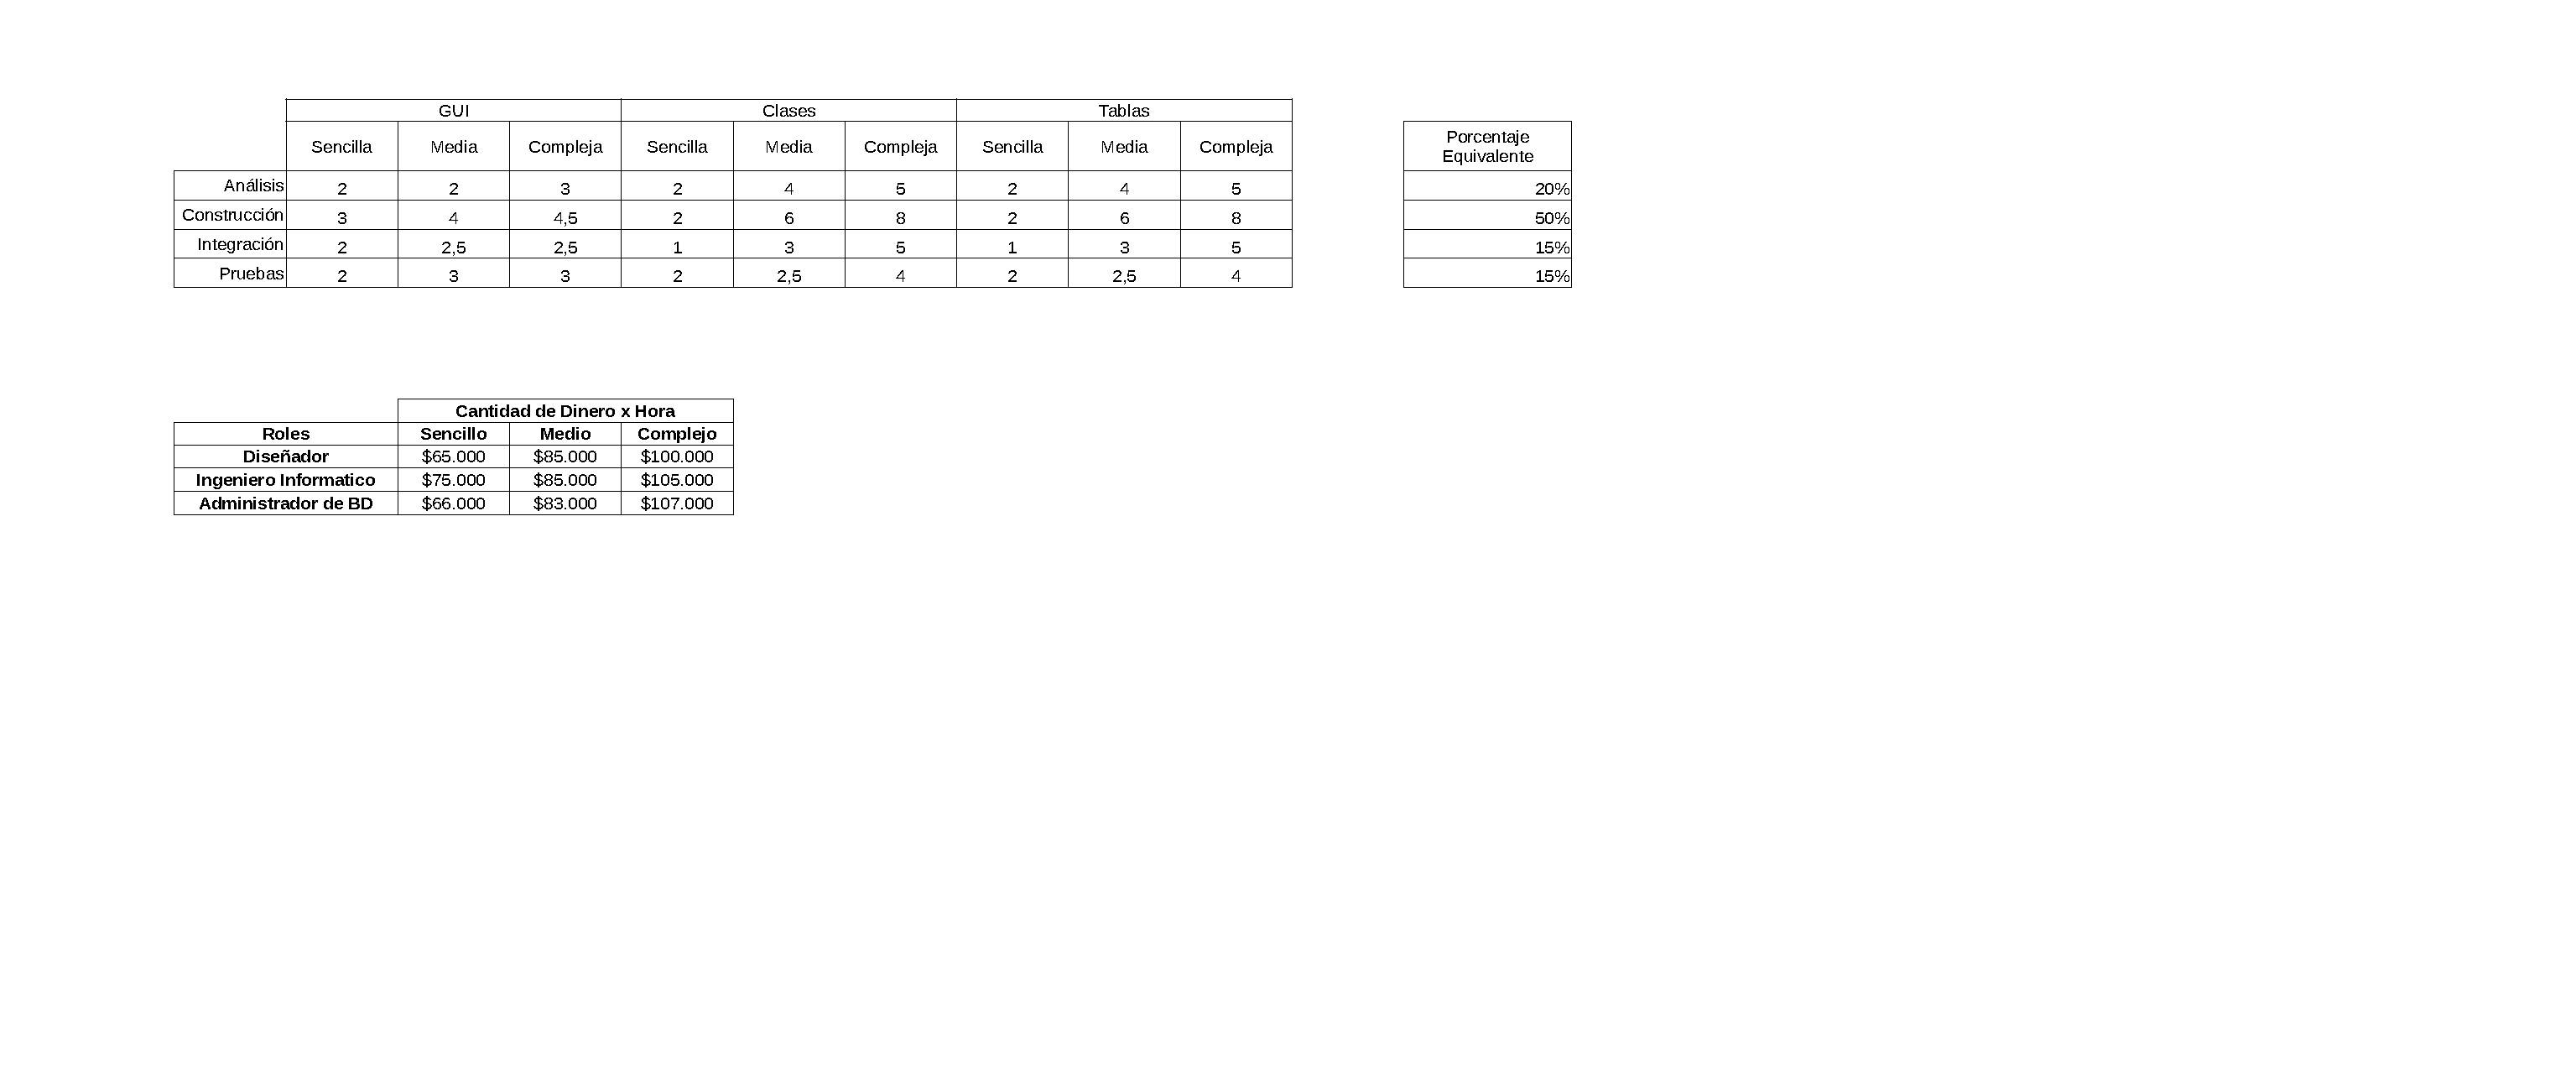
\includegraphics[width=1.2\linewidth]{libro/capitulo4/img/PROBE.pdf}
	\caption{Estimaci\'on}
\end{figure}


\section{Cronograma de Actividades}
\begin{figure}[h!]
	\centering
	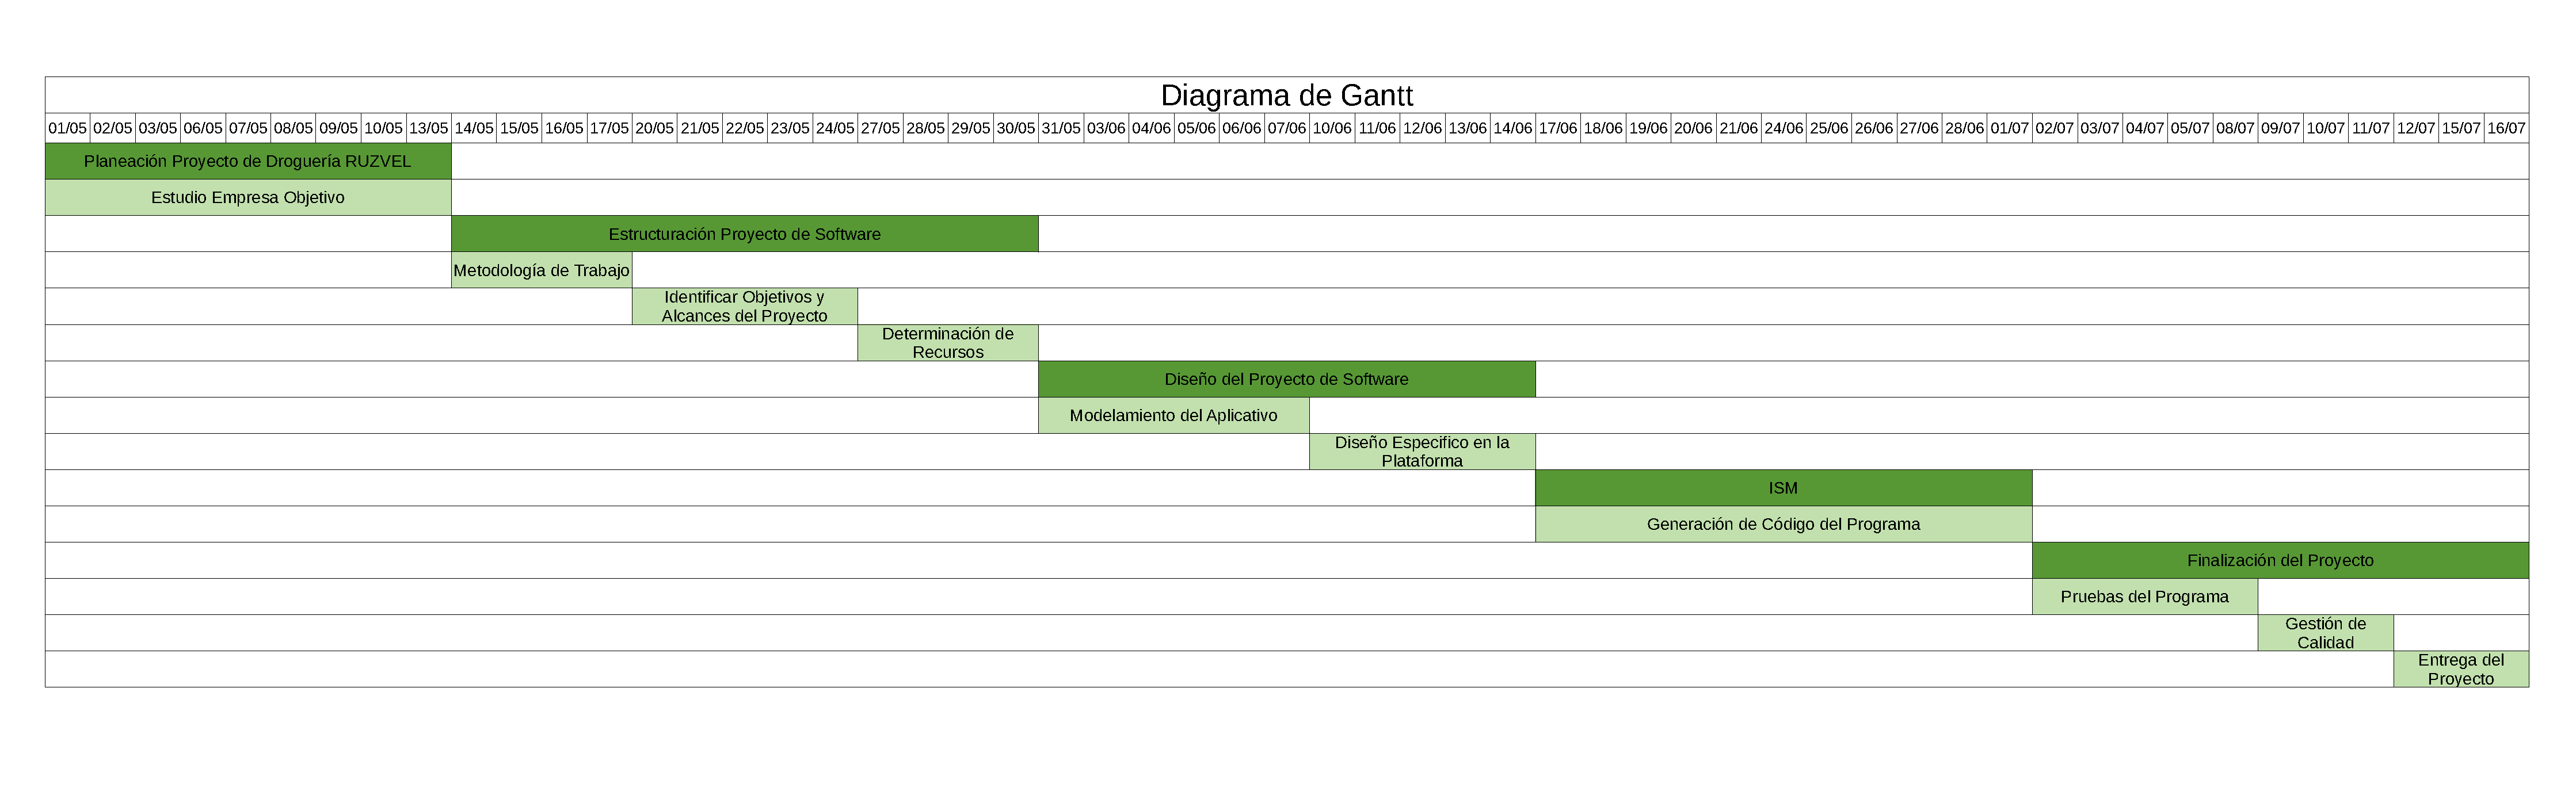
\includegraphics[width=0.8\linewidth]{capitulo4/img/Gantt.pdf}
	\caption{Diagrama de Gantt - Realizado mediante LibreOffice}
\end{figure}
